% vim:set et sw=2 ts=4 tw=72:
\chapter{Model}\label{chap:model}

This chapter introduces the \mt{} model and the algorithm used to
convert the DAG into the \mt{s}. Starting with an introduction of the
\mt{} model, the chapter includes the algorithm to convert the DAG into
\mt{s}, and an evaluation of that algorithm.

Thousands of commits are merged into the Linux kernel repository per
year.
Directly visualizing all of the information in a meaningful way is
difficult, or potentially impossible.
As shown in Figure~\ref{fig:linux_merge_distribution_per_release},
dividing the commits based on the merge into the master branch results
in groups that are relatively small;
the median size of the group being seven repository events.
The merge into the master branch is atomic, all of the context necessary
for integrating a commit is available at the merge into the master
branch.
Showing only the repository events that are are merged into the master
branch together filters the number of events down to a manageable size,
while still containing all of the information necessary to determine how
a commit is integrated, and the other commits integrated with it.

\evan{I'm confused about describing the \mt{} first, this is the
  description of what the tree is. I've tried to fix it, but I don't
  know what to fix.}

The \mt{} model is a tree structure,
rooted at the merge into the master branch.
The leaves of this tree are the commits and the merges are the inner
nodes.
The parent of a node is the next merge on the path to the root.
Merge trees are constructed recursively.
Starting at a commit, then walking up the children of the DAG until the
first merge is found.
All of the nodes that were traversed on the path to that merge are
children of the merge in the \mt{}.
Commits can be merged in multiple places.
The true parent of a commit in the tree is defined by shortest path.
In the case that there are the same number of intermediate nodes
between the commit and the root, time is used as a tie-breaker.
The structure recursively groups commits that are merged together,
making it easy to identify the commits that are integrated together.
Commits have a single path to reach the master branch, which makes
identifying the series of merges to the master branch and, in extension,
how the commit is integrated into the master branch of the master
repository.

The structure makes it easier to understand how commits are grouped and
integrated. This model simplifies and prunes the information from the
DAG, it also inverts the parent-child relationship. The parent of a node
in the DAG is the child of that node in the \mt{}.

In addition to identifying the path that a commit took to being merged,
the model enables easy aggregation of commit metadata at merges,
since the parent-child and child-parent relationship for each event
is known;
commits are aware of which merge is the next merge toward integration
into the master branch, and merges are aware of which commits are being
merged.

To illustrate this model I will use a small example: assume the commits
represented in Figure~\ref{fig:repoEvents} show the sequence of events
in a repository. The sequence starts with the initial commit in the
master branch of the master repository at time $t_0$. Repository event 1
is a commit, which gets forked into a separate repository, \textit{Repo
  A}, where another commit is made, event 2. Event 5 is a merge event,
merging event 2, 3, and 4 into \textit{Repo A}. Event 5 is branched
from, commit 6 happens in the new branch, while commit 7 is added
simultaneously to the original branch in \textit{Repo A}. Events 11 and
12 are both merge events, merging changes made in \textit{Repo A} into
the master branch of the master repository. As every repository is a
first-class repository, including local copies and forks, git does not
distinguish between forked repositories and branches, and in neither
case does it explicitly record where a commit was made. In this case,
commits are performed in various repositories and branches. The DAG
representation of these events is shown in Figure~\ref{fig:repoDAG}.

\begin{figure}[htbp]
  \centering
  \resizebox{0.8\textwidth}{!}{
  \begin{tikzpicture}[auto, on grid, semithick, state/.style={circle, text=black}]
    \foreach \x in {0, 1, 2, 3, 4, 5, 6, 7}
    \draw[shift={(\x + 0.5, -0.5)}, color=black] (0cm, 4cm) -- (0pt, -0.2cm);

    \node[state, draw=chartblue] (1) {1};
    \node[state, draw=chartyellow, above right= of 1] (2) {2};
    \node[state, draw=chartmagenta, above right= 2cm and 1cm of 2] (3) {3};
    \node[state, draw=chartblue, right= 2cm of 1] (4) {4};
    \node[state, draw=chartyellow, above right=of 4] (5) {5};
    \node[state, draw=chartred, above right=of 5] (6) {6};
    \node[state, draw=chartyellow, right=of 5] (7) {7};
    \node[state, draw=chartmagenta, above right= 2cm and 1cm of 7](8) {8};
    \node[state, draw=chartyellow, right= 2cm of 7] (9) {9};
    \node[state, draw=chartyellow, right=of 9] (10) {10};
    \node[state, draw=chartblue, below right=of 9] (11) {11};
    \node[state, draw=chartblue, below right=of 10] (12) {12};

    \draw (12) edge (11) edge[chartyellow] (10);
    \draw (11) edge (4) edge[chartyellow] (9);
    \draw (10) edge[chartyellow] (9);
    \draw (9) edge[chartmagenta] (8) edge[chartred] (6)
              edge[chartyellow] (7);
    \draw (8) edge[chartmagenta] (7);
    \draw (7) edge[chartyellow] (5);
    \draw (6) edge[chartred] (5);
    \draw (5) edge[chartmagenta] (3) edge[chartyellow] (2)
              edge[chartyellow] (4);
    \draw (4) edge (1);
    \draw (3) edge[chartmagenta] (2);
    \draw (2) edge[chartyellow] (1);

    \node [draw=chartblue, below = 1.5cm of 1] (l1) [thick, minimum height=0.8cm]{Master};
    \node [draw=chartyellow, below = 1.5 cm of 4] (l2) [thick, minimum height=0.8cm]{Repo A};
    \node [draw=chartred, below = 4.5cm of 8] (l3) [thick, minimum height=0.8cm]{Branch of Repo A};
    \node [draw=chartmagenta, below = 1.5 of 12] (l4) [thick, minimum height=0.8cm]{Repo B};

        \foreach \x in {0, 1, 2, 3, 4, 5, 6, 7, 8}
    \node[shift={(\x, -0.6)}, color=black] {$t_\x$};
  \end{tikzpicture}
}
  \caption{An example sequence of events performed in different
    repositories. The horizontal axis represents time. The branches and
    repositories are aligned horizontally, and color-coded. Each commit
    points to its parent. The initial commit is at time $t_0$, and the
    head is at $t_8$.}
  \label{fig:repoEvents}
%\vspace{-3mm}
\end{figure}

The commit nodes do not preserve branch information, which allows users
to rename branches and repositories without having to update the
preceding commits.
This is at the expense of maintain a consistent history.
It is desirable to reconstruct all of the branch and repository
information, shown in Figure~\ref{fig:repoEvents}, from the information
in the DAG, shown in Figure~\ref{fig:repoDAG}, but this may not be
possible.
Instead, I focus on determining the next merge that leads
toward the integration of a commit.
Depicted in Figure~\ref{fig:repoTree}, is the first version of the \mt{}.
It does not completely rebuild the lost information, but is able to
show the sequence of merges that a commit follows to be integrated,
and the commits that were involved with the integration.
This is the version of the \mt{} that is used in the visualizations, in
the construction of \tool{}, and in the user study.
This tree does not preserve the ordering of the commits within the
merge; however, the algorithm presented in Section~\ref{sec:algorithm}
preserves this information, but the visualizations in \tool{} do not
make use of it.

\begin{figure}[htbp]
  \centering
  \resizebox{0.8\textwidth}{!}{
  \begin{tikzpicture}[auto, on grid, semithick, state/.style={circle, text=black, black}]
    \node[state, black] (1) {1};
    \node[state, black, above right= of 1] (2) {2};
    \node[state, black, above right= 2cm and 1cm of 2] (3) {3};
    \node[state, black, right= 2cm of 1] (4) {4};
    \node[state, black, above right=of 4] (5) {5};
    \node[state, black, above right=of 5] (6) {6};
    \node[state, black, right=of 5] (7) {7};
    \node[state, black, above right= 2cm and 1cm of 7](8) {8};
    \node[state, black, right= 2cm of 7] (9) {9};
    \node[state, black, right=of 9] (10) {10};
    \node[state, black, below right=of 9] (11) {11};
    \node[state, black, draw=chartblue, below right=of 10] (12) {12};

    \draw (12) edge[-stealth] (11) edge[-stealth] (10);
    \draw (11) edge[-stealth] (4) edge[-stealth] (9);
    \draw (10) edge[-stealth] (9);
    \draw (9) edge[-stealth] (8) edge[-stealth] (6)
              edge[-stealth] (7);
    \draw (8) edge[-stealth] (7);
    \draw (7) edge[-stealth] (5);
    \draw (6) edge[-stealth] (5);
    \draw (5) edge[-stealth] (3) edge[-stealth] (2)
              edge[-stealth] (4);
    \draw (4) edge[-stealth] (1);
    \draw (3) edge[-stealth] (2);
    \draw (2) edge[-stealth] (1);
  \end{tikzpicture}
  }
  \caption{DAG representation of the commits represented in
    Figure~\ref{fig:repoEvents}. The DAG loses information about which
    repository the commit is performed in and through which merges it
    has passed on its way to the master branch. The DAG does not even
    distinguish the master branch from other branches.}
  \label{fig:repoDAG}
%\vspace{-3mm}
\end{figure}

\begin{figure}[htpb]
  \centering
  \resizebox{0.8\textwidth}{!}{
    \begin{tikzpicture}[auto, on grid, semithick, node distance=1cm, state/.style={circle, text=black, minimum size=7mm}]

      \node[state, draw=chartblue] (1) {1};
      \node[state, draw=chartblue, right=of 1] (4) {4};
      \node[state, draw=chartblue, right=of 4] (11) {11};
      \node[state, draw=chartblue, right=2.5cm of 11] (12) {12};

      \node[state, draw=chartyellow, above right= 1cm and 0.5cm of 11] (7) {7};
      \node[state, draw=chartyellow, above left= 1cm and 0.5cm of 11] (5) {5};
      \node[state, draw=chartyellow, right=of 7] (9) {9};
      \node[state, draw=chartyellow, left=of 5] (2) {2};
      \node[state, draw=chartmagenta, above=of 5] (3) {3};
      \node[state, draw=chartmagenta, above left=1cm and 0.5cm of 9] (6) {6};
      \node[state, draw=chartmagenta, above right=1cm and 0.5cm of 9] (8){8};
      \node[state, draw=chartyellow, above=of 12] (10) {10};

      \draw (11) edge[chartyellow, stealth-] (2) edge[chartyellow, stealth-] (5) edge[chartyellow, stealth-] (7) edge[chartyellow, stealth-] (9)
      (5) edge[chartmagenta, stealth-] (3)
      (9) edge[chartmagenta, stealth-] (6) edge[chartmagenta, stealth-] (8)
      (12) edge[chartyellow, stealth-] (10);
    \end{tikzpicture}
  }
  \caption{The \mt{s} computed for each commit in
    Figure~\ref{fig:repoDAG} showing the path that each commit takes to
    be merged into the master branch of the repository. This does not
    indicate how the events being merged are related. This figure
    retains the numerical order of the events, but the order is
    arbitrary.}
  \label{fig:repoTree}
\end{figure}

Using the depth of the node from the root of the tree, the branch
information is reconstructed. In our events, nodes 2, 5, 7, and 9, are
all on the same branch, and are merged into node 11. Nodes 5 and 9 are
merge nodes, 5 merges a single commit into the branch, and 9 merges two
nodes into the branch. In some cases, it is possible that a commit was
merged twice. In the case of node 9, it is merged into 11, though it
could also be merged into 12 through 10. The \mt{} is designed to use
the shortest distance in merges, and if two paths have the same distance
from the master branch, use the shortest distance through time.

\section{Algorithm}
\label{sec:algorithm}

Computing the \mt from a DAG for any repository may not be possible;
however, certain features of the development process of Linux make it
feasible to compute the \mt for the Linux repository. First, the master
branch of Linux is maintained by Linus Torvalds, and only Linus has
write access to it. This assertion is verified by
German~\cite{German2015}. The heuristic developed from this information
is presented in Algorithm~\ref{fig:alg}. In short, the algorithm first
identifies the commits made directly to the master branch, whereafter it
recursively determines the shortest path, using the DAG, from each
commit to the master branch using the inverted DAG\@.

\begin{algorithm}
        \caption{Computing the \mt of Linux from the DAG}\label{fig:alg}
        \begin{algorithmic}[1]
                \Function{ComputeMergeTree}{DAG}: tree
                % \State {\# Compute the tree from the DAG of Linux repository.}
                % \State {\# Returns $Tree$, a graph containing every commit }
                % \State {\# in DAG with the path it followed to master.}
                \State $head \gets \textit{Head of master of git repository}$
                \State $master \gets \textit{traverse DAG from head using }$
                \State \quad\quad\quad\quad $\textit{first parent until reaching root}$
                \State $nodes(Tree) \gets nodes(DAG)$
                \State \Function{MergeAtMaster}{cid}
                \State {\# Returns $(depth, merge, next)$}
                \State {\# Helper function}
                \State {\# Compute the closest merge into master, }
                \State {\# setting the children on the way to master.}
                \If {\textit{cid in master}}
                \State \Return $(0, cid, \varnothing)$
                \EndIf
                \State {$d \gets \infty$}
                \State {\# Traverse the inverted DAG}
                \For{$c \in children(cid, DAG)$}
                \State $(d_c, merge_c, next_c) \gets MergeAtMaster(c)$
                \If {$IsMerge(c)$}
                \State $fp \gets FindFirstParent(c)$
                \If {$fp \neq cid$}
                \State $d_c \gets d_c + 1$
                \State $next_c \gets c$
                \EndIf
                \EndIf
                \State {\# Find the shortest path}
                \If {$d_c < d$}
                \State $(d, m, next) \gets (d_c, merge_c, next_c)$
                \ElsIf{ $d_c = d$ }

                \State {\# Use the time as a tie-breaker}
                \If {$ cTime(merge_c) < cTime(m) $}
                \State $(m, next) \gets (merge_c, next_c)$
                \EndIf
                \EndIf
                \EndFor
                \State {\# $c$ is the commit that follows $cid$ on it's way to master}
                \State add edge $(cid, next)$ to $Tree$
                \State \Return $(d, m, next)$
                \EndFunction

                \State {\# Compute the distance for each commit discarding result}
                \For{$c \in nodes(DAG)$}
                \State $MergeAtMaster(c)$
                \EndFor
                \State \Return $Tree$
                \EndFunction
        \end{algorithmic}
\end{algorithm}

The algorithm is broken into two phases.
The first is determining which repository events happened on the master
branch.
This is done by traversing the first parent from the master branch
reference to the commit that has no parents.
The second phase is encompassed by the function
$MergeAtMaster$ which determines, for each commit, which merge the
commit is merged at, the depth (as variable $d$ in the algorithm), and
the next merge on the path to the master branch. The function
$MergeAtMaster$ has two parts, the first for determining the depth, from
the master branch, that the repository event is at. The second phase
determines the merge into the master branch, and the next merge on the
way to the master branch.
The distance is computed by shortest path close to the master branch as
possible.
If there is a tie between two paths, the path that merges into the
master branch sooner is taken.

An example is used to demonstrate the behaviour of the algorithm,
computing the merge at commit 5 in Figure~\ref{fig:repoEvents}.
$MergeAtMaster$, recurses along the children of the nodes it visits.
Eventually every child of every node along the path will be visited at
least once. Without loss of generality, suppose that the path recursed
along is from node 5 to 6, 9, 10, and finally 12.

The depth for each, except 12 (a merge into the master branch), is
initialized to infinity, the merge into master is blank, and the next
merge is blank. Merges into master trivially have a distance of 0 from
the master branch, and it merges itself into the master branch. The
recursion at 12 returns the triple $(0, \varnothing, 12)$ to the call
from 10. 12 is a merge commit and 10 is not the first parent, so the
temporary depth, $d_c$, is incremented to 1 and the temporary next
merge, $next_c$, is changed to 12. 1 is less than infinity, so the depth
is set to 1, the merge to 12, and the next to 12. This returns the
triple $(1, 12, 12)$ to the call from 9. 9 is the first parent of 10, so
no changes are made to the temporary variables.

The call to 9 recurses to the second child, 11. 11 is a merge into the
master so it returns $(0, \varnothing, 11)$ to the call from 9. 9 is not
the first parent of 11, so the $d_c$ is incremented to 1 and $next_c$ is
changed to 11. The distances $d_c$ and $d$ are the same, so time is used
to break the tie. 12 was merged after 11, so 11 replaces 12 as the
merge into the master branch for 9, as well as being the next merge. The
call for 9 returns the triple $(1, 11, 11)$ to the call for 6. 6 is not
the first parent of 9, so $d_c$ is incremented and $next_c$ is changed
to 9, as 9 merges 6. 2 is less than infinity, so the $d$ is changed to
2, the merge to 11, and the next merge to 9. The call to 6 returns the
triple $(2, 11, 9)$ to the call for 5.

The call for 5 recurses on the second child of 5, calling on 7, which
calls 8, and then 9. 9 can continue, but if the implementation of the
algorithm uses memoization, the call to 9 can immediately return the
triple $(1, 11, 11)$ to the call for 8, and avoid an exponential
runtime. 8 is not the first parent of 8, so $d_c$ is incremented to 2
and $next_c$ is changed to 9. 2 is less than infinity, so $d$ is changed
to 2, $merge$ to 11, and $next$ to 9. The call to 8 returns the triple
$(2, 11, 9)$ to the call for 7, which recurses on the second child of 7,
9. 9 returns the triple $(1, 11, 11)$. 7 is the first parent of 9, so
the depth is not incremented. $d_c$ is less than $d$, so $d$ is changed
to 1, $m$ to 11, and $next$ to 11, returning $(1, 11, 11)$ to the call
for 5. $d_c$ is less than $d$, so $d$ is changed to 1, $m$ to 11, and
$next$ to 11. There are no other children, so the function halts.

\section{Algorithm Evaluation}
\label{sec:algorithm_evaluation}

The merge trees generated by the algorithm must be validated to ensure
that they are an accurate representation of the events occurring in the
repository.
Evaluation poses some issues, as there is no easy way to accurately
gather this information directly from the DAG\@.
Further inspection of the merges provides some insight;
Linus Torvalds adds useful information about the
content of the merges.
For each branch being merged,
Linus includes either the first 20 commit titles and the total
number of commits being merged (see Figure~\ref{fig:sampleMerge}
for an example);
or if there are 20 or fewer commits being merged, the list of commit
titles.

\begin{figure}[htpb]
  \centering
\begin{textbox}
  \begin{verbatim}commit 3d30701b58970425e1d45994d6cb82f828924fdd
Merge: 8cbd84f2dd4e fd8aa2c1811b
Author: Linus Torvalds <torvalds@linux-foundation.org>
Date:   Tue Aug 10 15:38:19 2010 -0700

    Merge branch 'for-linus' of git://neil.brown.name/md

    * 'for-linus' of git://neil.brown.name/md: (24 commits)
      md: clean up do_md_stop
      md: fix another deadlock with removing sysfs attributes.
      md: move revalidate_disk() back outside open_mutex
      md/raid10: fix deadlock with unaligned read during resync
      md/bitmap:  separate out loading a bitmap from ...
      md/bitmap: prepare for storing write-intent-bitmap ...
      md/bitmap: optimise scanning of empty bitmaps.
      md/bitmap: clean up plugging calls.
      md/bitmap: reduce dependence on sysfs.
      md/bitmap: white space clean up and similar.
      md/raid5: export raid5 unplugging interface.
      md/plug: optionally use plugger to unplug an array ...
      md/raid5: add simple plugging infrastructure.
      md/raid5: export is_congested test
      raid5: Don't set read-ahead when there is no queue
      md: add support for raising dm events.
      md: export various start/stop interfaces
      md: split out md_rdev_init
      md: be more careful setting MD_CHANGE_CLEAN
      md/raid5: ensure we create a unique name for ...
      ...
  \end{verbatim}
\end{textbox}
  \caption{Example of how merges record a subset of commits being merged. The
                commit only shows the first 20 one-line summaries messages for the 24
                non-merge commits it merged. The ending ``\ldots'' is part of the log
                and represents that other commits were merged.}
  \label{fig:sampleMerge}
\end{figure}

This information is used to verify that the results of the \mt{}
algorithm are consistent with the information explicitly stated in the
merge log.
A program extracts the merges made by Linus into the master branch of
the repository.
The merges are gathered by two commands;\\
\verb|git log --merges --author='Linus Torvalds' v3.16| collects the
merges by Linus Torvalds, and
\verb|git log --format="%H" --first-parent --merges v3.16| collects the
merges that are along the master branch, assuming that the master branch
is not confounded.
The inner product of the results of the two commands leaves the set of
merges made by Linus Torvalds into the master branch.
The results of the algorithm were collected up to version 3.16, which is
why the set of merges must be limited to that version.
For each merge in the set of merges above, the program extracts the
number of commits, commit titles, commit date, authorship date from the
merge log and compares them against the corresponding generated \mt{}.

The results of the analysis found that 14670 merges along the master
branch were found in both the results of the \mt{} algorithm, and the
git logs. Two merges, \emph{186051d70444} and \emph{5170a3b24a91} were
found in the logs, but were not in the results of the algorithm, and 426
merges in the set of \mt{s}, but not in the logs.

Examining the two merges that were missing from the algorithm results,
assuming these merges are on the master branch means that there are also
situations where commits that were not made by Linus were added to the
master branch.
The graph for merge \emph{186051d70444} is shown in
Figure~\ref{fig:missing_merge}.
Knowing that Linus is the only one with direct merge access into the
master branch of the repository, the most plausible answer is that these
commits come from a fast-forward merge.
As git does not maintain the information necessary for distinguishing
commits added by a fast-forward merge from commits committed directly to
the branch, the only way to verify is to ask the person making the
merge, and given that these merges were made 13 years ago, the truth has
likely been lost to time.

\begin{figure}[htpb]
  \centering
  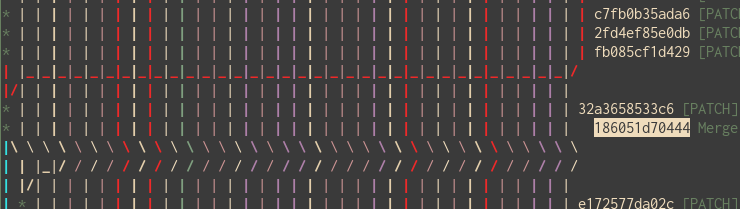
\includegraphics[width=0.8\linewidth]{Figures/model/18605.png}
  \caption{Merge \emph{186051d70444} graph view, showing that the merge
    into master is immediately followed(above) by a non-merging commit.}
  \label{fig:missing_merge}
\end{figure}

Conversely, many of the merges and commits that were in our database but
not found in the logs were due to the fast-forward merges. The commits
were detected as being part of the master branch when inserting the
commits into the database, but were not collected by our git log query
since they were not authored by Linus Torvalds.

Beyond investigating why merges show up in either the database or logs,
further analysis requires that the merges are present in both the
database and the merge log. There are 14198 merges with these
properties.

The results of the evaluation are summarized as follows:

\begin{itemize}
  \item

    Five merges did not have matching commit counts between the database
    and the logs. Upon further investigation, four merges had
    incorrectly formatted logs. The fifth merge,
    \emph{42a579a0f960}, is a \foxtrot{}
    merge. One commit is on the first-parent of the merge, and is
    therefore not detected when building the \mt{}, but is included
    in the merge log.

  \item

    The heuristic worked correctly until September 4, 2007, the earliest
    date that could be verified. Before this date, merge logs did not
    include a summary of the commits being merged, making it impossible
    to verify. Manual inspection indicates that the heuristic worked
    correctly for these commits, until December 12, 2006 where a
    \foxtrot{} merge occurs.

  \item

    There is 1 merge after September 4, 2007 that does not have recorded
    commit logs. This is due to incorrect formatting. If it were
    correctly formatted, it would report having 15 commits integrated,
    which is consistent with the results in the database.

  \item

    The algorithm breaks on merges prior to December 12, 2006 due to a
    foxtrot. There were 1537 merges made by Linus prior to this date.

  \item

    77 Merges were made by Linus into non-master branches after
    September 4, 2007. These merges were made into
    \emph{3f17ea6dea8b}, which is
    exceptionally large containing 7217 repository events, 6809 of
    which are commits, shown in Figure~\ref{fig:big_tree}.

\end{itemize}

\begin{figure}[htpb]
  \centering
  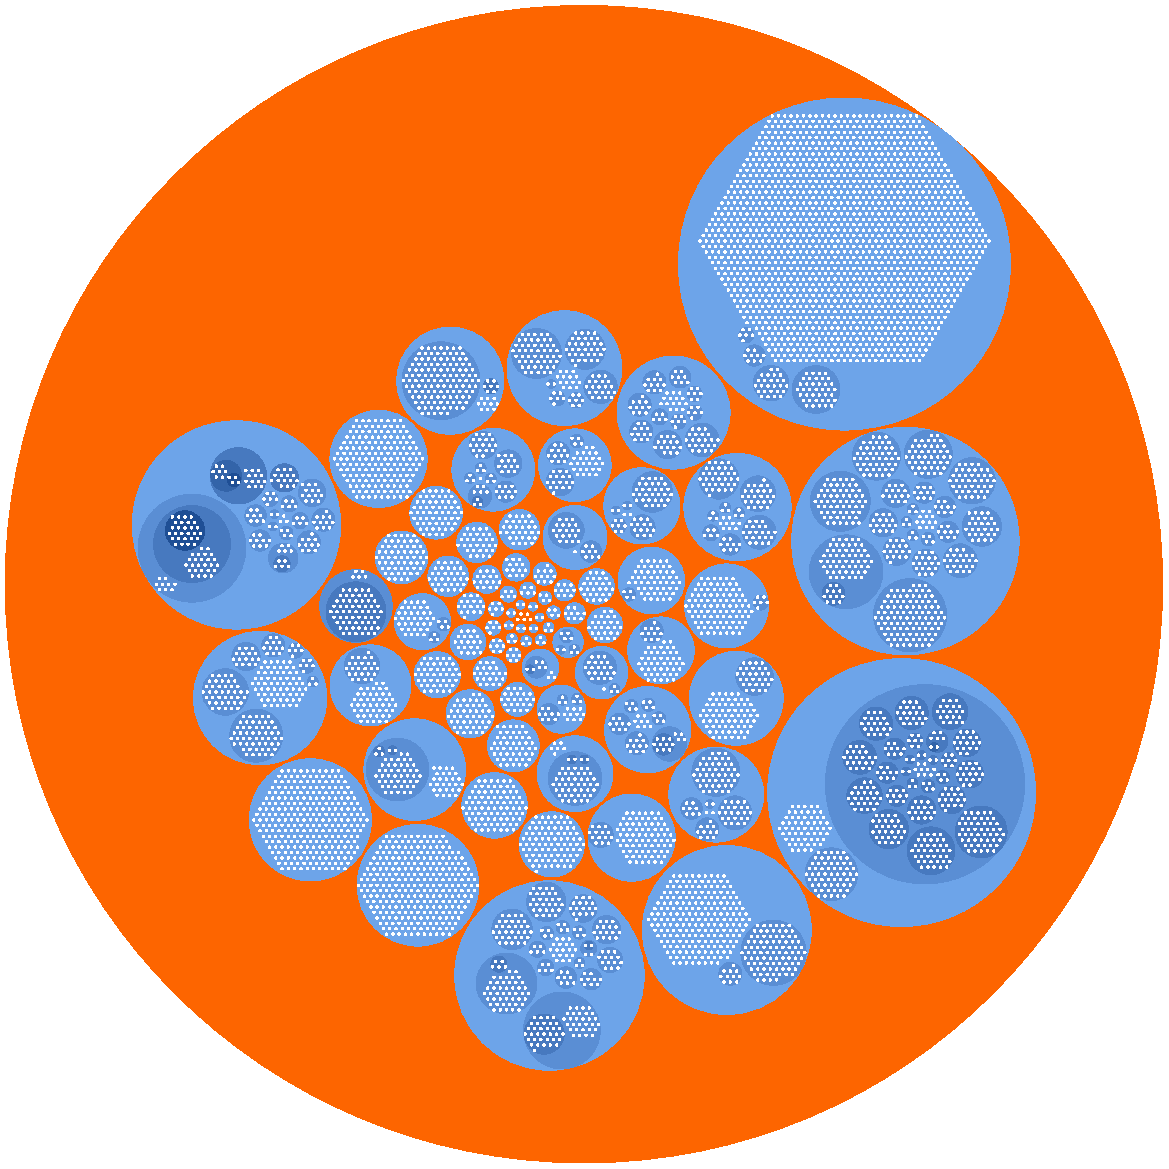
\includegraphics[width=0.8\linewidth]{Figures/model/big_tree.pdf}
  \caption{The largest \mt{}, made by Linus Torvalds into Linux 3.16.}
  \label{fig:big_tree}
\end{figure}

There were 12837 merges after September 4, 2007. With the exception of
the five merges, four with errors, and one as part of a \foxtrot{}, all
merges were correctly identified. The 835 merges between December 12,
2006, and September 4, 2007, appear to be correct, but cannot easily be
verified. The algorithm breaks on 1537 merges prior to December 12,
2006.
